\section{Requirement 2: stochastic multiple-campaigns environment}

% ============================================================
% Overview
% ============================================================
\begin{frame}{Stochastic multiple-campaigns environment}
    \begin{itemize}
        \item $N$ campaigns, each with its own ad valuation $v^{(i)}$, and joint highest-bid distribution $\mathcal{D}_{\mathbf{m}}$
        \item Single shared budget $B$ across \emph{all} campaigns
        \item Conflict graph $\mathcal{G}$: certain pairs of campaigns are mutually exclusive (cannot win both)
        \item Action per round: choose $N$ bids, one for each campaign, from a bid space $\mathcal{B}$ of size $K$ $\implies K^N$ possible superarms
        \item Algorithm to be studied: \textbf{Combinatorial-UCB} with budget
        \begin{itemize}
            \item Its output is a distribution $\gamma$ for the probability of choosing each superarm
        \end{itemize}
    \end{itemize}
\end{frame}

% ============================================================
% Conflicts graph
% ============================================================

\begin{frame}{Conflict graph - model}
    A graph in which:
    \begin{itemize}
        \item each node represents a campaign
        \item an edge between two nodes represents a conflict between incompatible campaigns, meaning that they cannot be bid on during the same round (but both can be bid on in different rounds)
    \end{itemize}

    \centering
    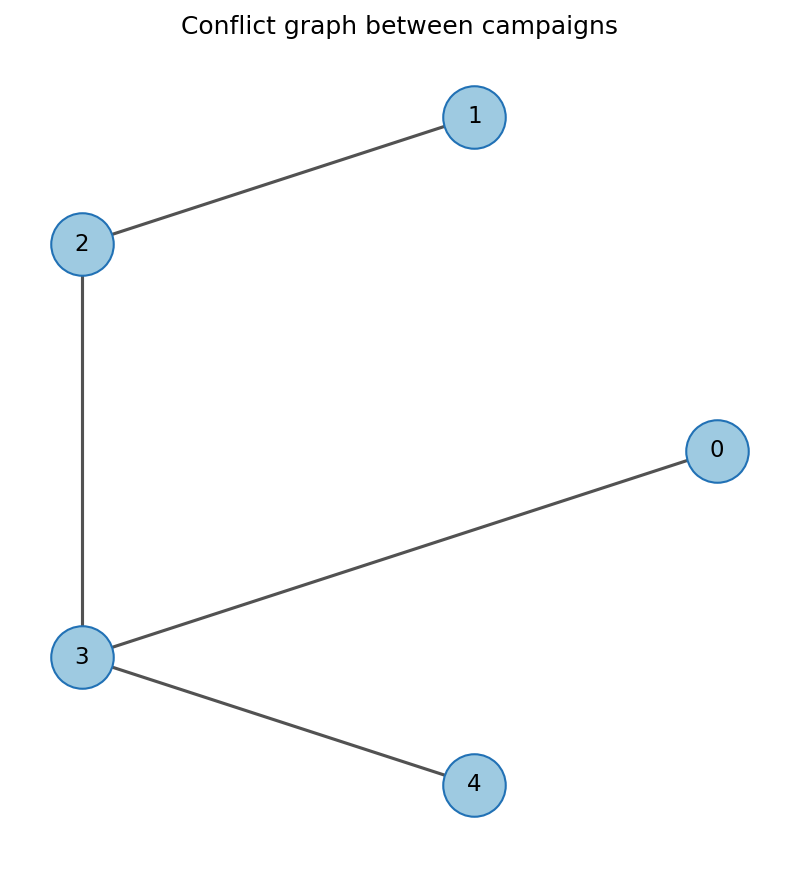
\includegraphics[width=0.26\textwidth]{figures/req2_conflict_graph.png} $\qquad$
    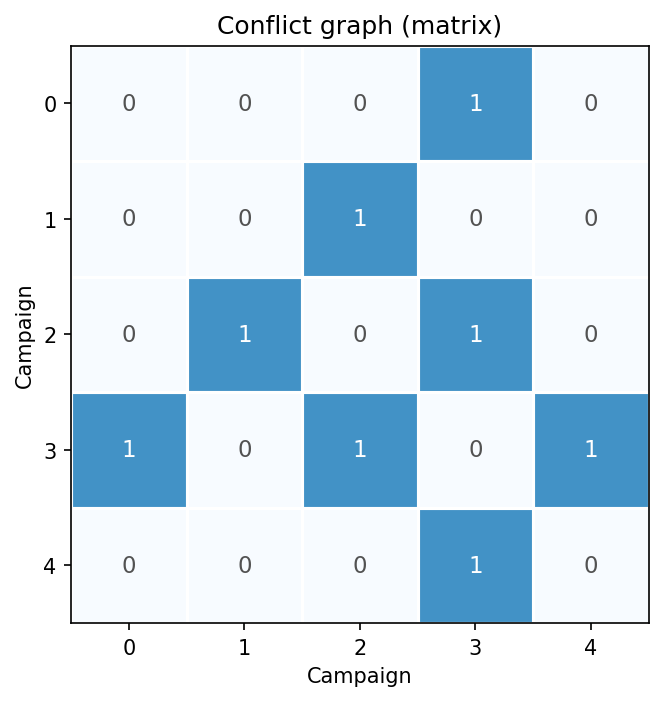
\includegraphics[width=0.25\textwidth]{figures/req2_conflict_matrix.png}

\end{frame}

% ============================================================
% Why uncorrelated / correlation comment
% ============================================================
\begin{frame}{Joint distribution of competing bids}
    \begin{itemize}
        \item Simplest model: per-campaign highest competing bid $m_t^{(i)} \sim \mathrm{Beta}(n_i, 1)$, sampled independently
        \begin{itemize}
            \item Corresponds to each competitor bidding independently of others, even across campaigns
            \item The joint distribution between all the campaigns can be defined by simply multiplying the product of the independent probabilities corresponding to a set of highest competing bids
        \end{itemize}
        \item Reality: fully-joint distribution $\mathcal{D_\mathbf{m}}$ which models correlations among the highest competing bids $\mathbf{m}$ of the campaigns 
        \begin{itemize}
            \item This is because each competitor may bid across multiple campaigns, introducing correlations (common budget, common objective, common market condition)
            \item In this case, the joint distribution cannot be decomposed into single-campaign distribution
        \end{itemize}
    \end{itemize}

    \begin{block}{}
        \textbf{Do we really need to model correlations between campaigns?}
    \end{block}
\end{frame}

\begin{frame}{Structural decomposition of the utilities and costs}
    \textbf{Assumption:} Without loss of generality, we consider the same ad valuation for all the campaigns $\implies$ the bid space $\mathcal{B}$ is identical (same available bids for all the campaigns)

    \vspace{0.5cm}

    \begin{itemize}
        \item At every round, we choose one superarm $\mathbf{b} = (b_1,\ldots,b_N) \in \mathcal{B}^N \sim \gamma$ and the environment chooses the highest competing bids $\mathbf{m} = (m_1,\ldots,m_N) \sim \mathcal{D}_\mathbf{m}$ for each campaign

        \item We observe a utility $f^{(i)}(b_i, m_i)$ for each campaign; the total utility $f(\mathbf{b}, \mathbf{m})$ received is the sum of the per-campaign utilities: 
        \[ f(\mathbf{b}, \mathbf{m}) = \sum_{i=1}^N f^{(i)}(b_i, m_i) \]
    \end{itemize}
\end{frame}

\begin{frame}{Structural decomposition of the utilities and costs}
    \begin{itemize}
        \item The expected utility $\bar{f}(\gamma)$ for any superarm distribution $\gamma$ and joint highest-competing-bid distribution $\mathcal{D}_\mathbf{m}$ is 
        \[\bar{f}(\gamma) = \mathbb{E}_{\mathbf{b} \sim \gamma}\left[ \mathbb{E}_{(m^{(1)}, \cdots, m^{(N)}) \sim \mathcal{D_\mathbf{m}}}\left[ \sum_{i=1}^N f^{(i)}(b_i, m_i) \right] \right]\]

        \item By linearity of expectation,
        \[\bar{f}(\gamma) = \sum_{i=1}^N \mathbb{E}_{\mathbf{b} \sim \gamma}\left[ \mathbb{E}_{(m^{(1)}, \cdots, m^{(N)}) \sim \mathcal{D_\mathbf{m}}}\left[ f^{(i)}(b_i, m_i) \right] \right]\]
    \end{itemize}
\end{frame}

\begin{frame}{Structural decomposition of the utilities and costs}
    \begin{itemize}
        \item Since each $f^{(i)}$ only depends on the highest competing bid in that same campaign,
        \[\bar{f}(\gamma) = \sum_{i=1}^N \mathbb{E}_{\mathbf{b} \sim \gamma}\left[ \mathbb{E}_{m^{(i)} \sim \mathcal{D}_{\mathbf{m}_i}}\left[ f^{(i)}(b_i, m_i) \right] \right] = \sum_{i=1}^N \bar{f}^{(i)}(\gamma)\]
        with $\mathcal{D}_{m_i}$ being the \underline{\textbf{marginalized}} distribution for the highest competing bid $m_i$ of campaign $i$ and $\bar{f}^{(i)}(\gamma)$ being its utility for the current action distribution $\gamma$ over superarms.

        $\implies$ correlations among the highest competing bids of all campaigns disappear!
    \end{itemize}
\end{frame}

\begin{frame}{Structural decomposition of the utilities and costs}
    \begin{alertblock}{Takeaway}
        A joint model having correlations between the highest competing bids $m_1,\ldots,m_N$ is not inherently more expressive than a model that independently samples the highest competing bids of the campaigns according to their marginal probabilities according to the joint model, \textbf{as far as it concerns our quantities of interest, because they are linear}.
    \end{alertblock}

    $\implies$ We can simply model (and also sample) the highest-competing-bid distributions of the campaigns independently!

    \vspace{0.5cm}
    
    A few notes:
    \begin{itemize}
        \item The same also holds for the expected cost $\bar{c}(\gamma)$ 
        \item This means that we can consider separate values of $f^{(i)}(b_i)$ and $c^{(i)}(b_i)$ (or of their estimates) for each bid $b_i$ of every campaign $i$, like we did in the single-campaign setting!
    \end{itemize}
\end{frame}

% ============================================================
% Clairvoyant LP
% ============================================================
\begin{frame}{Clairvoyant}
    \begin{itemize}
        \item A clairvoyant "in expectation":
        \begin{itemize}
            \item the highest competing bids $m_t$ are stochastic and sampled from a distribution $\mathcal{D}_m$ \\
            $\implies$ we need the best behavior \emph{on average}
            \item the clairvoyant only needs to satisfy the budget constraint \emph{in expectation}, but is allowed to exceed per-round budget at any round
        \end{itemize}
        
        \begin{block}{Assumption} 
        The clairvoyant knows the underlying distribution $\mathcal{D}_m$ of the highest competing bids $m_t$, but not their actual realizations!
        \end{block}
    \end{itemize}
\end{frame}

\begin{frame}[fragile]{Clairvoyant}
    \begin{itemize}
        \item A clairvoyant "in expectation":
        \begin{itemize}
            \item the highest competing bids $m_t$ are stochastic and sampled from a distribution $\mathcal{D}_m$ \\
            $\implies$ we need the best behavior \emph{on average}
            \item the clairvoyant only needs to satisfy the budget constraint \emph{in expectation}, but is allowed to exceed per-round budget at any round
        \end{itemize}
        
        \begin{block}{Assumption} 
        The clairvoyant knows the underlying distribution $\mathcal{D}_m$ of the highest competing bids $m_t$, but not their actual realizations!
        \end{block}
    \end{itemize}

    \begin{tikzpicture}[remember picture, overlay]
        \node[
            draw=red,          % Border color (remove or change to white if needed)
            fill=white,         % Box background color
            thick,              % Thick border line
            minimum width=12cm,          % Set the exact width
            minimum height=6.75cm,         % Set the exact height
            text width=10cm,
            rounded corners,    % Rounded edges for the box
            inner sep=10pt,      % Padding inside the box around the text
            align=center
        ] at (current page.center) {
            Conceptually, the same as the single-campaign clairvoyant! \\
            \\
            However, now we have \emph{multiple campaigns}... \\
            \\
            What is the optimal strategy?
        };
  \end{tikzpicture}
\end{frame}

\begin{frame}{The apparent difficulty: the superarm space}
    \begin{itemize}
        \item A superarm is a complete vector of bids:
        \[\mathbf b=(b_1,\ldots,b_N).\]

        \item With \(K=|\mathcal B|\) possible bids per campaign,
        the number of possible superarms is
        \[|\mathcal B|^N = K^N.\]

        \item A generic clairvoyant policy would therefore be a distribution
        \[\gamma(\mathbf b), \qquad \mathbf b\in\mathcal B^N.\]

        \item This is exponentially large in the number of campaigns and polynomially large in the number of bids.
    \end{itemize}

    \begin{block}{}
        \textbf{We have already removed the correlations in the highest competing bids! Can we also avoid optimizing over the full joint distribution?}
    \end{block}
\end{frame}

\begin{frame}{Why randomization over campaign subsets is necessary}
    Consider two conflicting campaigns \(i\) and \(j\).

    \begin{center}
    \begin{tabular}{c|cc}
        & Expected per-round utility & Expected per-round cost \\ \hline
        \(i\) & \(0.7\) & \(0.4\) \\
        \(j\) & \(0.5\) & \(0.2\)
    \end{tabular}
    \end{center}

    \vspace{0.3cm}

    Per-round budget: $\rho=0.3.$

    Since \(i\) and \(j\) are in conflict, they cannot be active simultaneously.
\end{frame}

\begin{frame}{Strategies without randomization}
    \begin{block}{Deterministic choice: campaign \(i\)}
        To meet the budget constraint, randomize only between bidding on $i$ (with probability $p$) and not bidding:
        \[0.4 \cdot p + 0 \cdot (1 - p) \le 0.3 \quad \Longrightarrow \quad p \le 0.75.\]
        Hence
        \[\bar{f}(\text{bidding only on } i) = 0.7 \cdot 0.75 = \boxed{0.525}.\]
    \end{block}

    \begin{block}{Deterministic choice: campaign \(j\)}
        Campaign \(j\) can always be played:
        \[\bar{f}(\text{bidding only on } j) = \boxed{0.5}.\]
    \end{block}
\end{frame}

\begin{frame}{Randomization over campaign subsets improves the optimum}
    Now randomize between the two feasible campaign subsets $\{i\}$ and $\{j\}$: choose
    \[\{i\}\text{ with probability } p,\qquad\{j\}\text{ with probability } 1 - p.\]

    The expected per-round cost of the randomization is
    \[0.4 \cdot p + 0.2 \cdot (1 - p).\]

    Using the full budget:
    \[0.4 \cdot p + 0.2 \cdot (1 - p) = 0.3 \quad \Longrightarrow \quad p = 0.5.\]

\end{frame}

\begin{frame}{Randomization over campaign subsets improves the optimum}
    Therefore, the expected per-round utility from randomizing over subsets $\{i\}$ and $\{j\}$ is
    \[R = 0.7 \cdot 0.5 + 0.5 \cdot 0.5 = 0.35 + 0.25 = \boxed{0.6 > 0.525}.\]

    \begin{alertblock}{Conclusion}
        There exists at least one setting in which randomization over feasible subsets is strictly better than any deterministic choice, even when randomization is already allowed within a campaign
    \end{alertblock}
    $\implies$ We cannot choose a single deterministic subset of campaigns on which to bid in every round: our algorithm must keep a distribution over the subsets!
\end{frame}

\begin{frame}{What can we decompose?}
    As we have seen, linearity lets us decompose $\bar{f}(\gamma)$ and $\bar{c}(\gamma)$, ignoring correlations in the competing bids, for example:

    \[\bar{f}(\gamma) = \sum_{i=1}^N \mathbb{E}_{\mathbf{b} \sim \gamma}\left[ \mathbb{E}_{m^{(i)} \sim \mathcal{D}_{\mathbf{m}_i}}\left[ f^{(i)}(b_i, m_i) \right] \right]\]
     
    \begin{block}{}
        \textbf{Can we also ignore correlations in the joint distribution between our bids, i.e. can we simply learn one independent distribution for each campaign, sample these and then form a joint action using the sampled actions?}
    \end{block}
\end{frame}

\begin{frame}{What can we decompose?}
    $\implies$ No! Campaigns are coupled by the conflict graph, and an independent decomposition cannot model all possible joint policies. Consider two conflicting campaigns $i, j$ and their single-bid distributions $\gamma^{(i)}, \gamma^{(j)}$:
    \begin{enumerate}
        \item if we allow both their $\gamma^{(i)}$ and $\gamma^{(j)}$ to bid a non-zero value, we end up violating the conflict
        \item if we constrain all the probability mass of either $\gamma^{(i)}$ or $\gamma^{(j)}$ to the $0.0$ bid, we permanently lose the possibility of bidding over that campaign
    \end{enumerate}
\end{frame}

\begin{frame}{The right abstraction: factorizing the joint probability}
    What can we do then?

    Let $S \subseteq \{1, \ldots, N\}$ be a subset of campaigns on which we bid in a round.
    \begin{itemize}
        \item Separate the superarm $\mathbf{b}$ into:
        \begin{enumerate}
            \item which campaigns are active;
            \item which bid is used for each active campaign.
        \end{enumerate}

        \item A feasible superarm can then be represented as
        \[a = (S,\mathbf b_S),\]
        where $S$ is an conflict-free subset of campaigns and
        $\mathbf{b}_S = (b_i \in \mathcal B \sim \gamma_{i | S}$ for every $i \in S)$, with $\gamma_{i | S}$ being the distribution over the bids of campaign $i$ when the subset $S$ is played.

        \item The expected utility and cost for any subset $S$ are additive:
        \[\bar{f}(S) = \sum_{i \in S} \bar{f}^{(i)}(\gamma_{i|S}), \qquad \bar{c}(S) = \sum_{i \in S} \bar{c}^{(i)}(\gamma_{i|S}).\]
    \end{itemize}
\end{frame}

\begin{frame}{The right abstraction: factorizing the joint probability}
    \begin{itemize}    
        \item We can do for $\mathbf{b}$ what we did earlier for $\mathbf{m}$ in the expression for $\bar{f}(\gamma)$ (same for $\bar{c}(\gamma)$):
        \begin{equation*}
            \begin{aligned}
                \bar{f}(S) &= \sum_{i \in S} \mathbb{E}_{\mathbf{b} \sim \gamma}\left[ \mathbb{E}_{m^{(i)} \sim \mathcal{D}_{\mathbf{m}_i}}\left[ f^{(i)}(b_i, m_i) \right] \right] \\
                &= \sum_{i \in S} \mathbb{E}_{b_i \sim \gamma_{i|S}}\left[ \mathbb{E}_{m^{(i)} \sim \mathcal{D}_{\mathbf{m}_i}}\left[ f^{(i)}(b_i, m_i) \right] \right]
            \end{aligned}
        \end{equation*}
    \end{itemize}

    \begin{block}{}
        This means that, even though we cannot ignore overall correlations in the distribution over the full superarms due to the conflict graph, we can at least ignore the correlations in the distribution over bids once we have fixed a feasible subset of campaigns! 
    \end{block}
    $\implies$ the full joint distribution $\gamma = \mathbb{P}\left[ \mathbf{b} \right]$ over the competing bids
    is not needed to evaluate the expected utility/cost of a superarm!
\end{frame}

\begin{frame}{The right abstraction: factorizing the joint probability}
    \begin{itemize}
        \item But: \textbf{the distribution over feasible superarms is still necessary} to encode the conflict graph and randomize across campaign subsets.

        \vspace{0.2cm}

        $\implies$ "post-select" between campaigns by factorizing the joint distribution $\gamma$, i.e. $\mathbb{P}\left[ \mathbf{b} \right] = \mathbb{P}\left[ S, \mathbf{b}_S \right]$. Using the definition of conditional probability and the fact that we can ignore intra-subset correlations among bids of different campaigns, we have
        \[\mathbb{P}\left[ S, \mathbf{b}_S \right] = \mathbb{P}\left[ S \right] \mathbb{P}\left[ \mathbf{b}_S | S \right] = \mathbb{P}\left[ S \right] \prod_{i \in S}\mathbb{P}\left[ b_i | S \right]\]

        We can thus define a two-step sampling procedure for the joint action:
        \begin{enumerate}
            \item sample a conflict-free subset $S$ of campaigns from a distribution $\gamma_s = \mathbb{P}\left[ S \right]$ over all the feasible subsets;
            \item sample one bid for each campaign from the conditional distributions $\gamma_{i|S} = \mathbb{P}\left[ b_i | S \right]$.
        \end{enumerate} 
    \end{itemize}
\end{frame}

\begin{frame}{Clairvoyant formulation: factorized distribution}
    \vspace{-0.2cm}
    
    \footnotesize\begin{equation*}
        \begin{aligned}
            \gamma_s^\star, [\gamma_i]^\star = \arg & \max_{\gamma_s \in \mathbb{R}^{2^N}, [\gamma_{i|S}] \in \mathbb{R}^{NK}} ~~~ \sum_S \sum_{i \in S} \sum_b \textcolor{red}{\gamma_s(S) \gamma_{i|S}(b)}\, \bar{f}^{(i)}(b) \\
            & \begin{aligned} 
                \text{s.t.} ~~~~~~~~~~~~~~~~~~ & \sum_S \sum_{i \in S} \sum_b \textcolor{red}{\gamma_s(S) \gamma_{i|S}(b)}\, \bar{c}^{(i)}(b) \le \rho \quad & \text{(budget)} \\
                & \sum_S \gamma_s(S) = 1 & \text{(subset probability)} \\
                & \sum_b \gamma_{i|S}(b) = 1 \quad \forall S, i & \text{(conditional probability)} \\
                & \gamma_{i|S}(0) = 0 \quad \forall S,\, \forall i \in S & \text{(campaign in subset)} \\
                & \gamma_{i|S}(0) = 1 \quad \forall S,\, \forall i \notin S & \text{(campaign not in subset)} \\
                & \gamma_s(S) = 0 \quad \forall S \text{ having conflicts} & \text{(conflict)} \\
                & 0 \le \gamma_s(S) \le 1 \quad \forall S \\
                & 0 \le \gamma_{i|S}(b) \le 1 \quad \forall b 
            \end{aligned}
        \end{aligned}
    \end{equation*}

    $\implies$ \textcolor{red}{Non-linear Program!}
\end{frame}

\begin{frame}{Clairvoyant formulation: factorized distribution}
    \footnotesize Redefine the LP variables into $\gamma_{S, i}(b)$ to use the joint probability $\mathbb{P}\left[ S, b_i \right] = \gamma_s(S) \gamma_{i|S}(b)$ instead (same amount of variables) $\implies$ \textcolor{red}{Linear Program!}

    \vspace{-0.2cm}
    
    \footnotesize\begin{equation*}
        \begin{aligned}
            \gamma_s^\star, [\gamma_i]^\star = \arg & \max_{\gamma_s \in \mathbb{R}^{2^N}, [\gamma_{S, i}] \in \mathbb{R}^{NK}} ~~~ \sum_S \sum_{i \in S} \sum_b \textcolor{red}{\gamma_{S, i}(b)}\, \bar{f}^{(i)}(b) \\
            & \begin{aligned} 
                \text{s.t.} ~~~~~~~~~~~~~~~~~~ & \sum_S \sum_{i \in S} \sum_b \textcolor{red}{\gamma_{S, i}(b)}\, \bar{c}^{(i)}(b) \le \rho \quad & \text{(budget)} \\
                & \sum_S \gamma_s(S) = 1 & \text{(subset probability)} \\
                & \textcolor{red}{\sum_b \gamma_{S, i}(b) = \gamma_S(S) \quad \forall S, i} & \textcolor{red}{\text{(marginalization)}} \\
                & \textcolor{red}{\gamma_{S, i}(0)} = 0 \quad \forall S,\, \forall i \in S & \text{(campaign in subset)} \\
                & \textcolor{red}{\gamma_{S, i}(0)} = 1 \quad \forall S,\, \forall i \notin S & \text{(campaign not in subset)} \\
                & \gamma_s(S) = 0 \quad \forall S \text{ having conflicts} & \text{(conflict)} \\
                & 0 \le \gamma_s(S) \le 1 \quad \forall S \\
                & 0 \le \textcolor{red}{\gamma_{S, i}(b)} \le 1 \quad \forall b 
            \end{aligned}
        \end{aligned}
    \end{equation*}
\end{frame}

\begin{frame}{Clairvoyant: what $\gamma^\star$ over subsets of campaigns looks like}
    \centering
    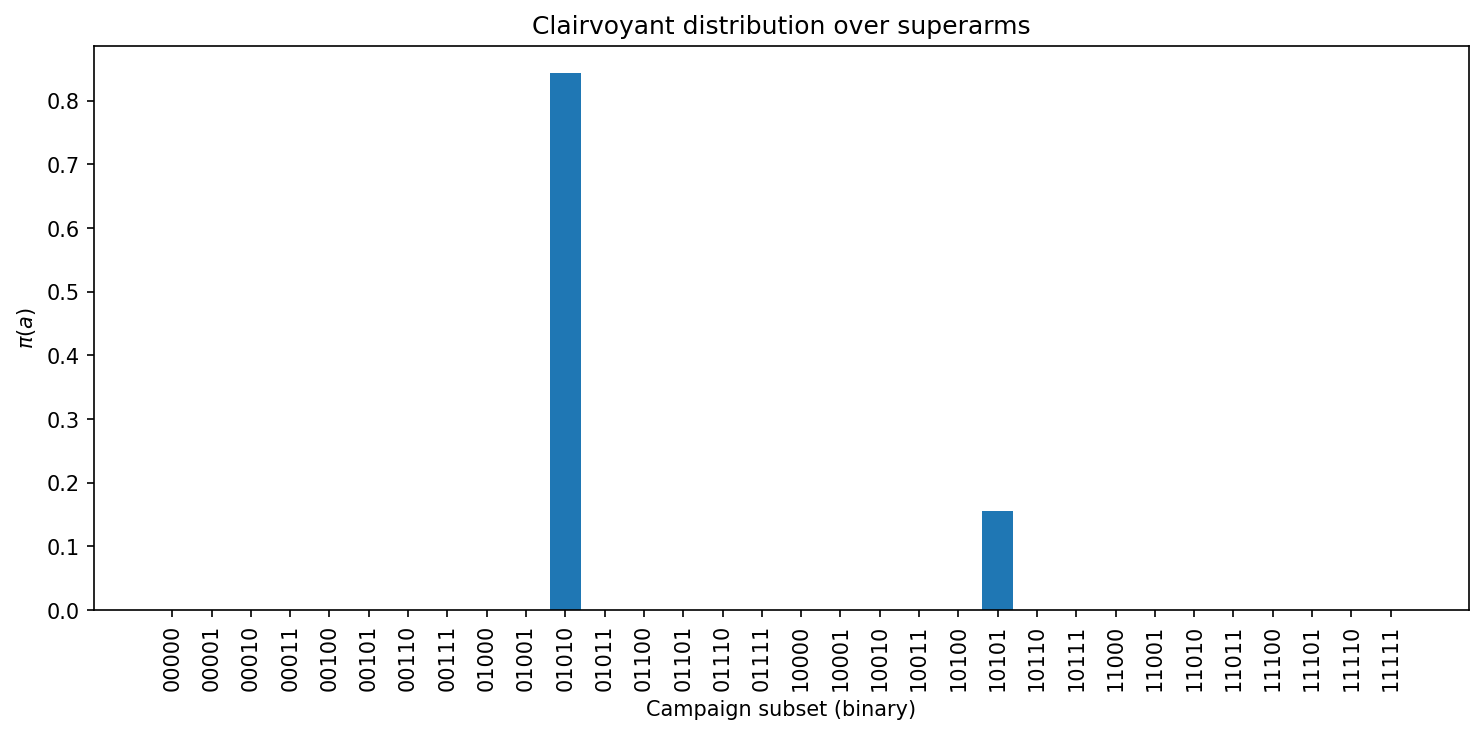
\includegraphics[width=0.8\textwidth]{figures/req2_true_clairvoyant_superarm_distribution.png}\\
    \scriptsize
    A randomized distribution over all the subsets of campaigns optimized by the clairvoyant of Requirement 2. We do not show the conditional distributions over bids within the single campaigns, since they can differ from one subset to another.
\end{frame}

% ============================================================
% Combinatorial-UCB
% ============================================================
\begin{frame}{Combinatorial-UCB: algorithm}
    Implements the UCB-like bidding approach for a combinatorial set of joint actions (i.e., bids on multiple campaigns)

    
    \begin{block}{Core idea}
        \vspace{-0.5cm}
        \[\boxed{\text{UCB estimates} \> + \> \text{conflict-aware campaigns subset optimization} \> + \> \text{budget constraint}}\]
    \end{block}

    \vspace{0.2cm}

    \begin{itemize}
        \item \textbf{Exploration rounds (first $K$ rounds):} randomly-chosen feasible superarms, aiming to explore as many arms as possible
        \begin{itemize}
            \item Some arms might not be chosen $\implies$ no problem, confidence radius gets set to 1 so that they will be explored afterwards
        \end{itemize}
        \item \textbf{Action selection:} we could, as in the single-campaign setting, solve the same LP as the clairvoyant and then sample a bid from the resulting optimal distribution...
    \end{itemize}
\end{frame}

\begin{frame}{Combinatorial-UCB: simpler approach}
    \footnotesize...but it's kinda expensive to do that \emph{every single round}! Instead, we split the clairvoyant LP into two suboptimal (but simpler) Linear Programs:
    \begin{itemize}
        \item First, we solve the single-campaign LP from Requirement 1 with per-round budget $\rho$ to obtain an optimal distribution $\gamma^{(i)}$ over bids for each campaign;
        \item Then, we use the solutions $\gamma^{(i)}$ to form expected utilities/costs for each campaign, and we select a distribution $\gamma_s^\star$ over campaigns subsets through the following LP over all the campaign subsets:
    \end{itemize}

    \vspace{-0.2cm}

    \footnotesize\begin{equation*}
        \begin{aligned}
            \gamma_s^\star = \arg & \max_{\gamma_s \in \mathbb{R}^{2^N}} ~~~ \sum_S \gamma_s(S) \left(\sum_{i \in S} \bar{f}^{(i)}(\gamma^{(i)})\right) \\
            & \begin{aligned} 
                \text{s.t.} ~~~~~~~~~ & \sum_S \gamma_s(S) \left(\sum_{i \in S} \bar{c}^{(i)}(\gamma^{(i)})\right) \le \rho \quad & \text{(budget)} \\
                & \sum_S \gamma_s(S) = 1 & \text{(subset probability)} \\
                & \gamma_s(S) = 0 \quad \forall S \text{ having conflicts} & \text{(conflict)} \\
                & 0 \le \gamma_s(S) \le 1 \quad \forall S \\
            \end{aligned}
        \end{aligned}
    \end{equation*}
\end{frame}

\begin{frame}{True clairvoyant against simplified clairvoyant}
    \begin{alertblock}{}
        We can also use this approach to build a clairvoyant; however, experimental results show that this approach achieves a little less expected utility than the true clairvoyant that we explained earlier
        $\implies$ for this reason, we use this approach only in the Combinatorial-UCB algorithm, but we keep the true clairvoyant for computing the regret
    \end{alertblock}

    \vspace{0.2cm}
    
    \centering
    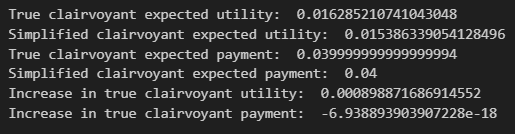
\includegraphics[width=0.6\textwidth]{figures/req2_true_clairvoyant_against_simplified_clairvoyant.PNG}
\end{frame}

% ============================================================
% Splitting the problem
% ============================================================
\begin{frame}{Explosion of LP variables}
    \centering
    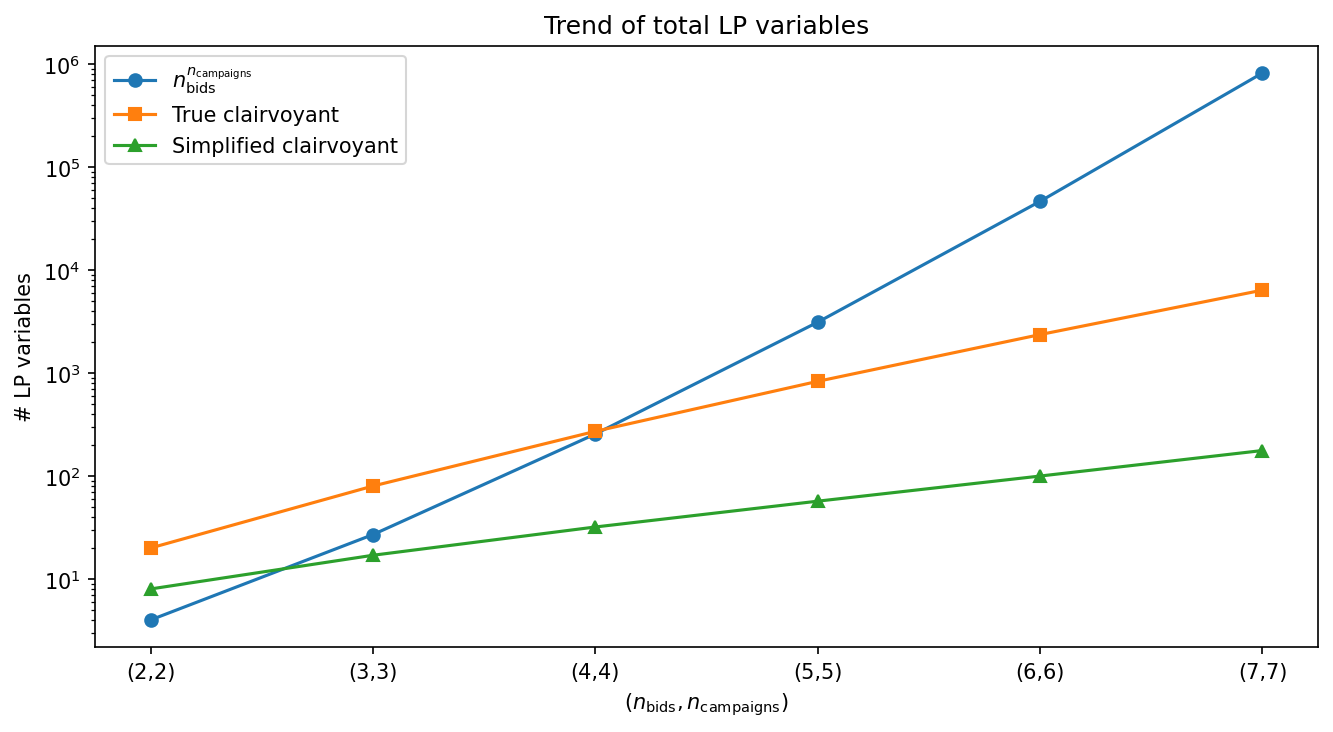
\includegraphics[width=0.7\textwidth]{figures/req2_lp_variables_trend.png}\\
    \scriptsize
    Comparison of the variables in the three possibilities for the LP: \textcolor{blue}{full joint distribution} (LP not analyzed in these slides), \textcolor{orange}{distribution from true clairvoyant}, \textcolor{green}{distribution from simplified clairvoyant}. Note that the y-axis is logarithmic.
\end{frame}

% ============================================================
% Results
% ============================================================
\begin{frame}{Results: Combinatorial-UCB using true LP}
    \begin{columns}[T]
        \begin{column}{0.6\textwidth}
            \centering
            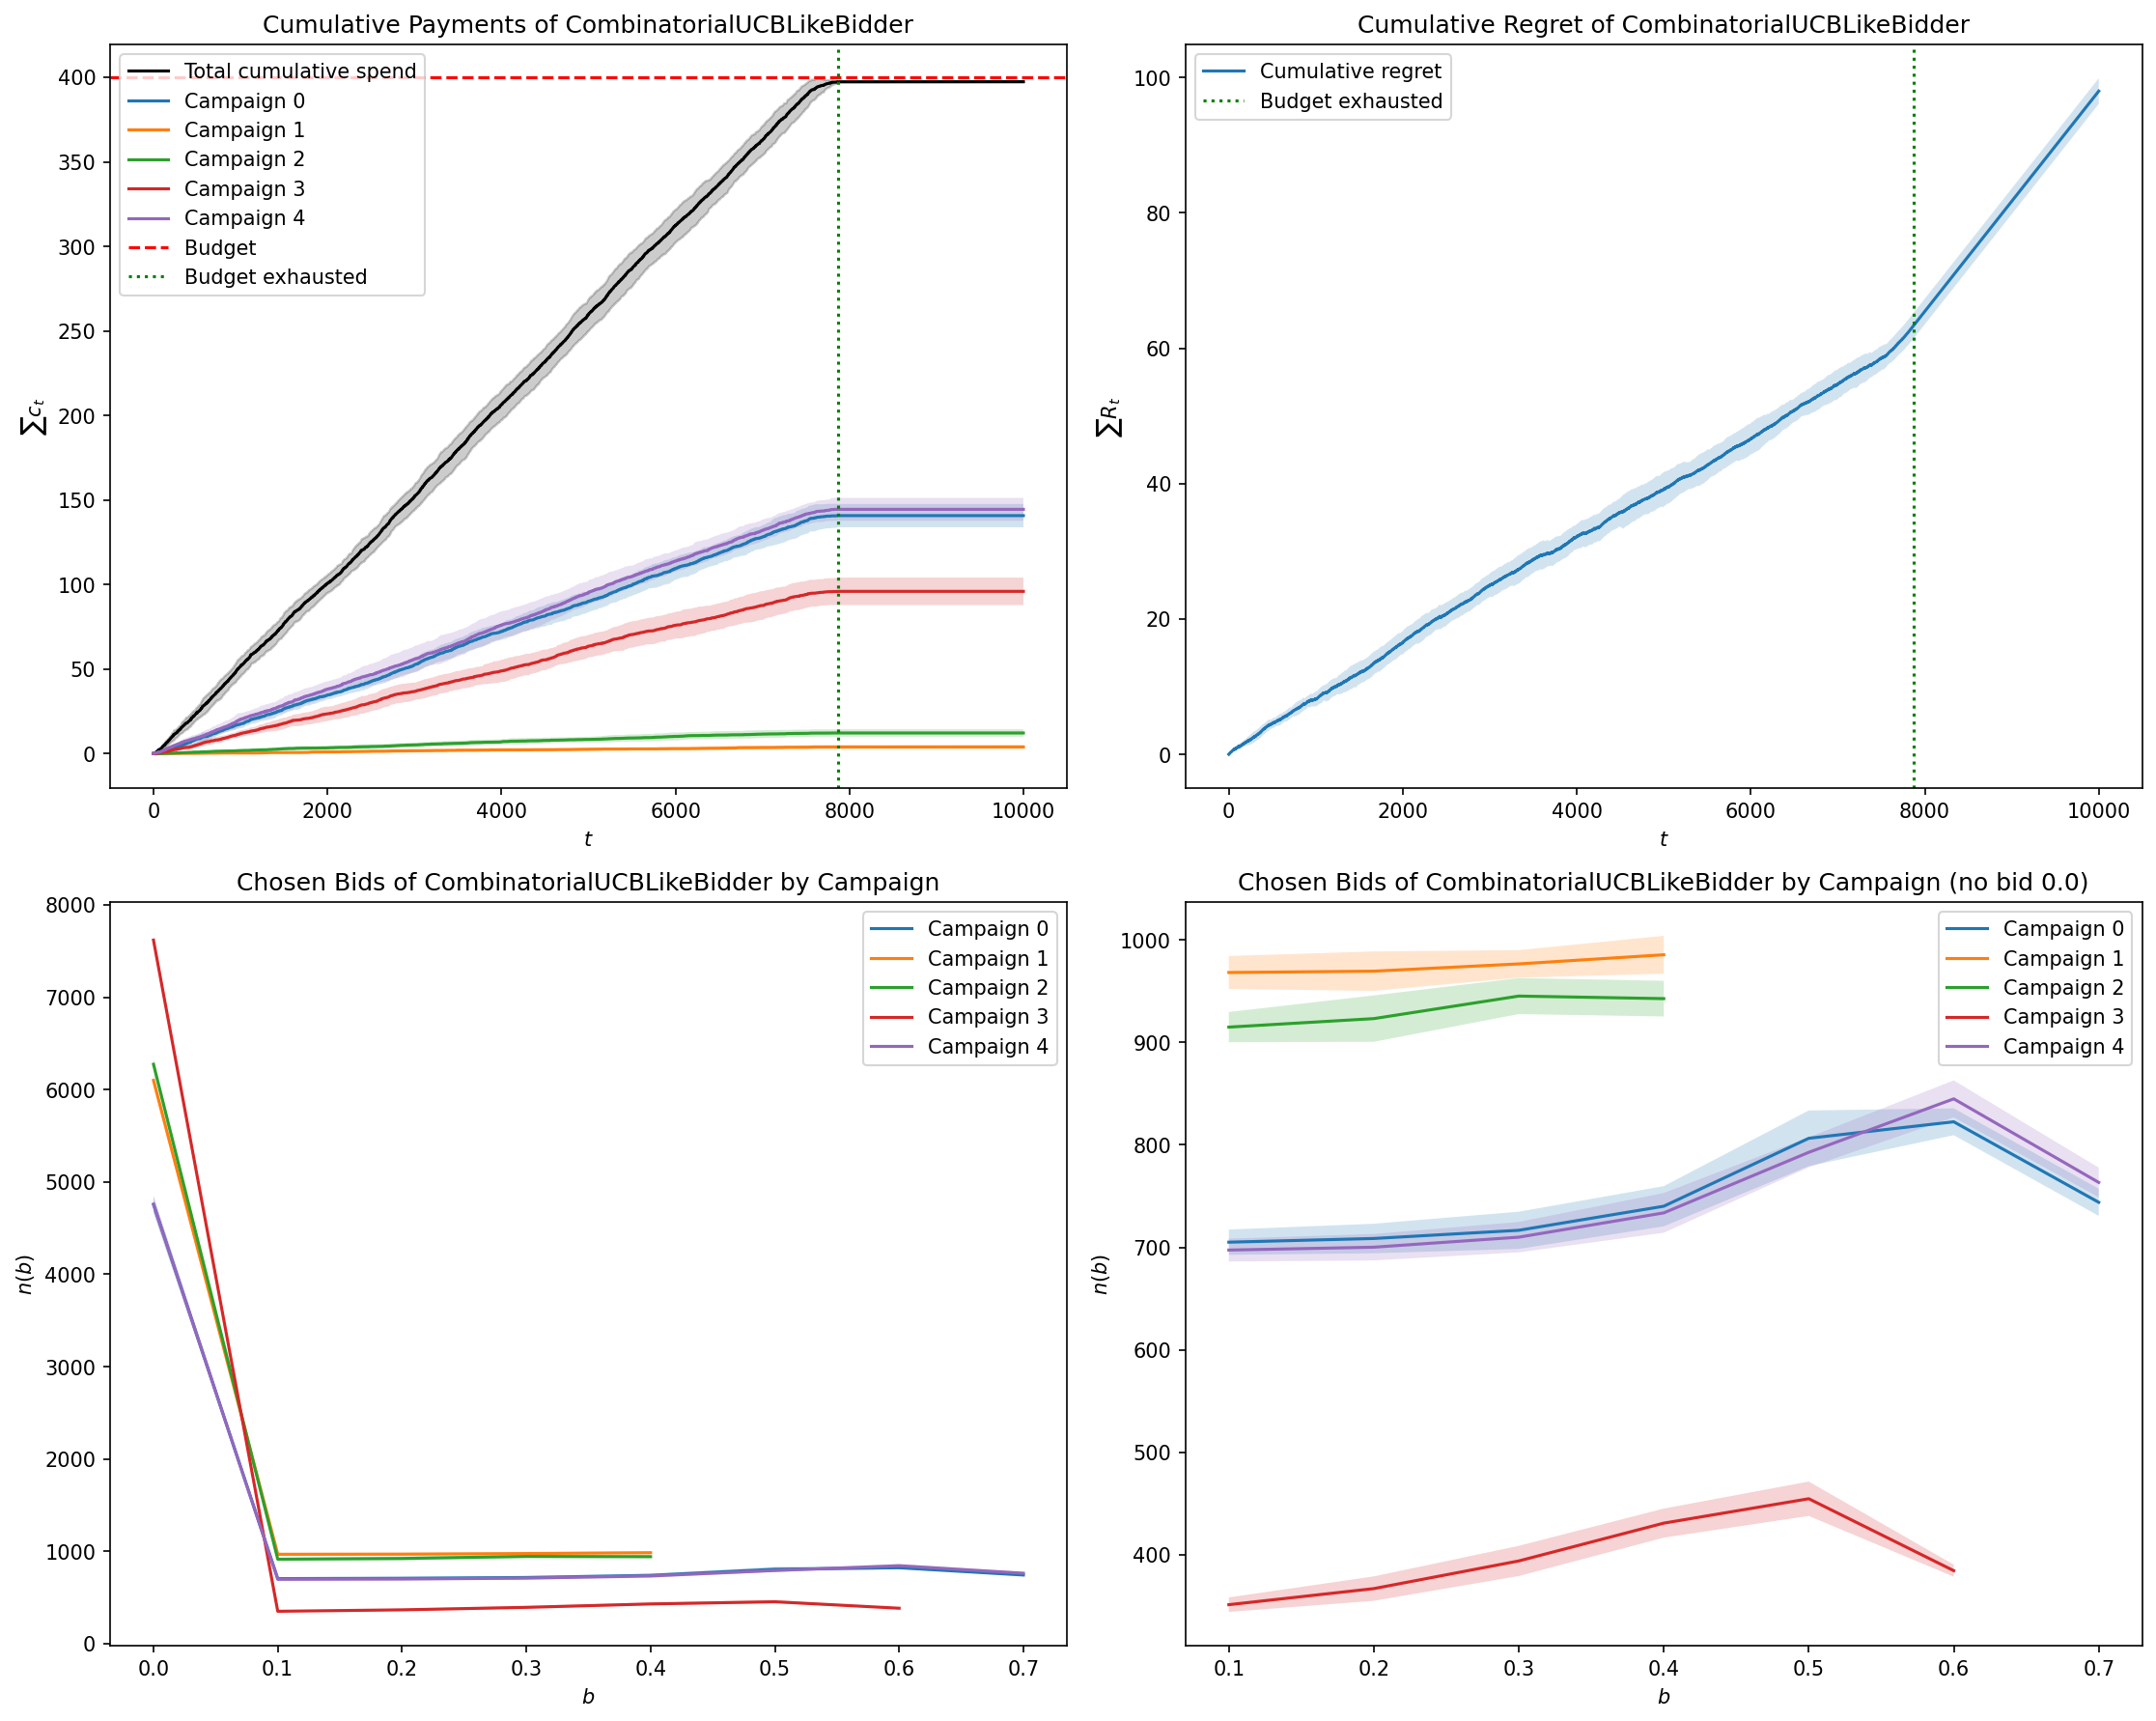
\includegraphics[width=0.9\textwidth]{figures/req2_true_true_experiment_results.png}\\
        \end{column}
        \begin{column}{0.3\textwidth}
             \begin{itemize}
                \item $10000$ (!) rounds are not enough to get evident sublinear regret and a clear separation among bids, although a hint of a peak among the bids of some campaigns can be seen
                \item Randomizing among subsets of campaigns leads to each campaign not being played sometimes
            \end{itemize}
        \end{column}\hfill
    \end{columns}
\end{frame}

\begin{frame}{Results: Combinatorial-UCB using simplified LP}
    \begin{columns}[T]
        \begin{column}{0.6\textwidth}
            \centering
            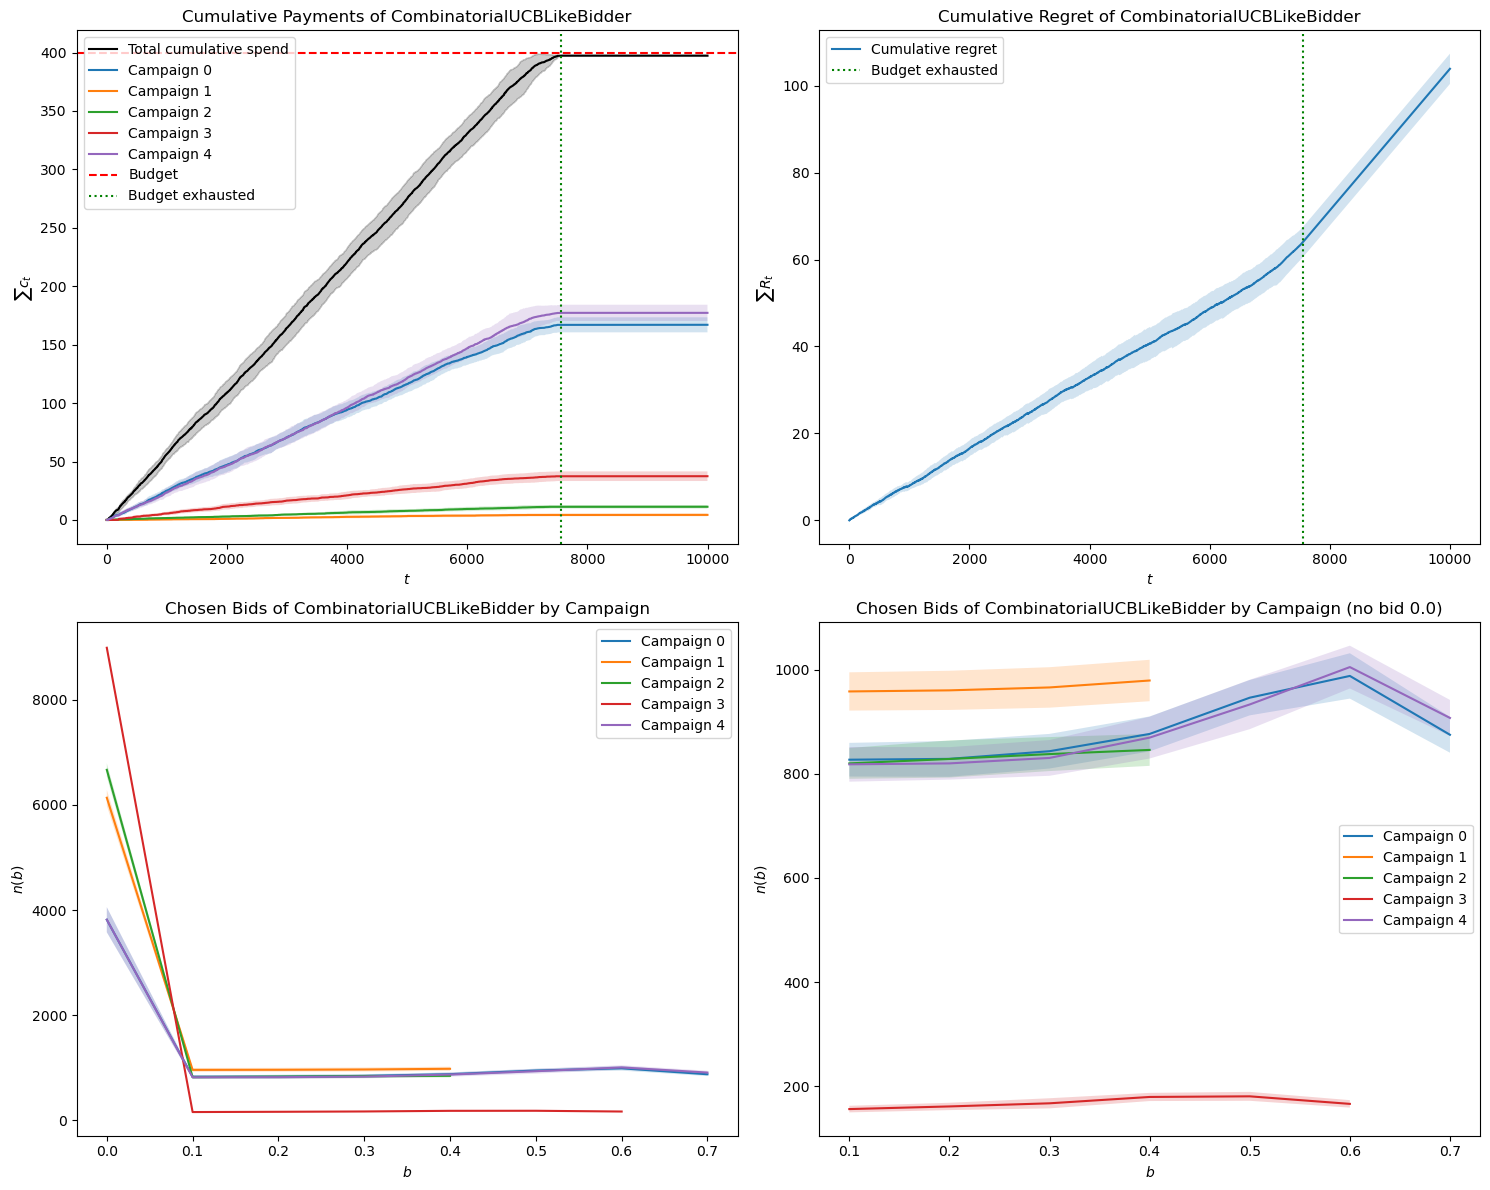
\includegraphics[width=0.9\textwidth]{figures/req2_simplified_true_experiment_results.png}\\
        \end{column}
        \begin{column}{0.3\textwidth}
             \begin{itemize}
                \item The regret is similar to that achieved using the true LP
                \item The separation between bids played is even less clear
            \end{itemize}
        \end{column}\hfill
    \end{columns}
\end{frame}

\begin{frame}{Results: comparison of the regrets of the two variants}
    \centering
    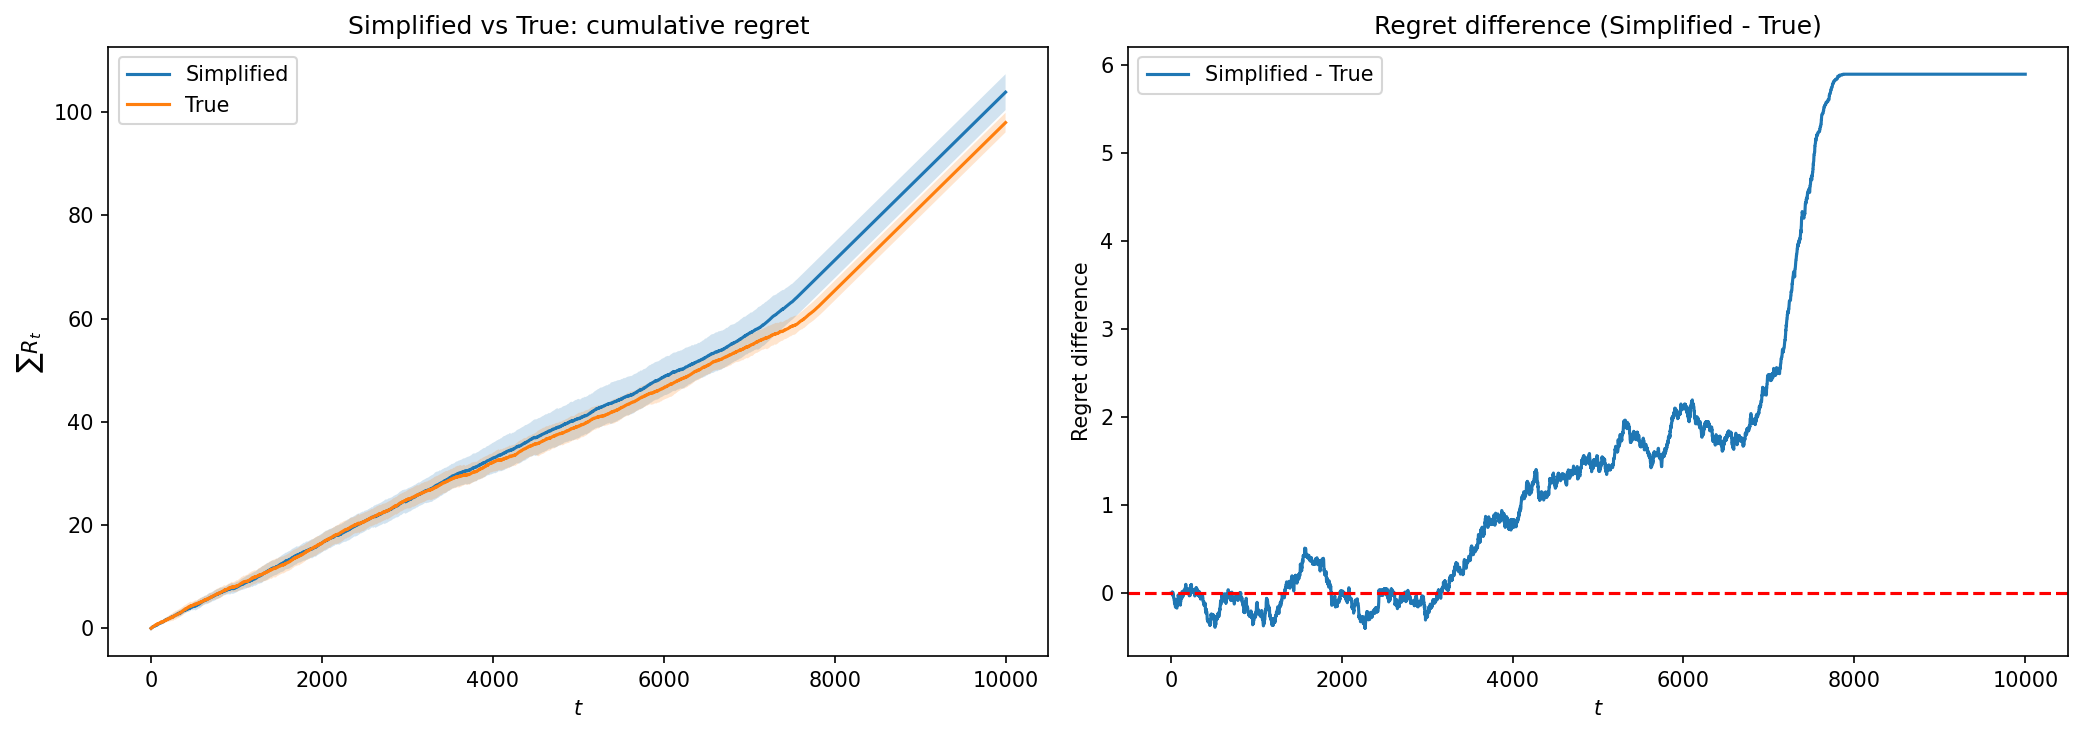
\includegraphics[width=\textwidth]{figures/req2_simplified_vs_true_regret.png}\\
    \scriptsize
    The Combinatorial-UCB bidder that uses the true LP achieves a little less regret than the bidder using the simplified LP (but also takes three times as much time to execute $\implies$ probably not worth it!).
\end{frame}
